\documentclass[10pt,journal,compsoc]{IEEEtran}

\ifCLASSOPTIONcompsoc
  \usepackage[nocompress]{cite}
\else
  % normal IEEE
  \usepackage{cite}
\fi
\usepackage{algorithm}
\usepackage{algpseudocode}
\usepackage{verbatim}
\usepackage{amsmath}
\usepackage{amssymb}
\usepackage{graphicx}
\usepackage{bbm}
\usepackage{listings}

\newtheorem{theorem}{Theorem}[section]
\newtheorem{lemma}[theorem]{Lemma}
\newtheorem{proposition}[theorem]{Proposition}
\newtheorem{corollary}[theorem]{Corollary}
\newenvironment{proof}[1][Proof]{\begin{trivlist}
		\item[\hskip \labelsep {\bfseries #1}]}{\end{trivlist}}
\newenvironment{definition}[1][Definition]{\begin{trivlist}
		\item[\hskip \labelsep {\bfseries #1}]}{\end{trivlist}}
\newenvironment{example}[1][Example]{\begin{trivlist}
		\item[\hskip \labelsep {\bfseries #1}]}{\end{trivlist}}
\newenvironment{remark}[1][Remark]{\begin{trivlist}
		\item[\hskip \labelsep {\bfseries #1}]}{\end{trivlist}}
\newcommand{\qed}{\nobreak \ifvmode \relax \else
	\ifdim\lastskip<1.5em \hskip-\lastskip
	\hskip1.5em plus0em minus0.5em \fi \nobreak
	\vrule height0.75em width0.5em depth0.25em\fi}


\hyphenation{op-tical net-works semi-conduc-tor}
\begin{document}
\title{Joint Embedding of Graphs}
\author{Shangsi Wang,
        Carey E. Priebe,
        Joshua T. Vogelstein,
        Avanti Athreya,
        Minh Tang,
        Vince Lyzinski,
        Youngser Park
         
%\IEEEcompsocitemizethanks{\IEEEcompsocthanksitem Shangsi Wang was with the Department of Applied Mathematics and Statistics, Johns Hopkins University,MD, 21218.\protect\\E-mail: swang127@jhu.edu
%\IEEEcompsocthanksitem Shangsi Wang was with the Department of Applied Mathematics and Statistics, Johns Hopkins University,MD, 21218.}}
%\thanks{Manuscript received April 19, 2005; revised August 26, 2015.}
}


% The paper headers
%\markboth{Journal of \LaTeX\ Class Files,~Vol.~14, No.~8, August~2015}%
%{Shell \MakeLowercase{\textit{et al.}}: Bare Demo of IEEEtran.cls for %Computer Society Journals}



\IEEEtitleabstractindextext{
\begin{abstract}
In this paper, we propose a method to jointly embed multiple undirected graphs. The method identifies a linear subspace spanned by rank one symmetric matrices and projects adjacency matrices of graphs into the subspace. The embedding coefficients can be treated as features of graphs. We propose a random graph model which can be used to model multiple random graphs. It can be shown that under the model our method produces estimates of parameters with small errors. We demonstrate through simulation experiments that our joint embedding method leads to state of the art performance for inference on multiple graphs. We further conduct a real data experiment which shows that an individual creativity index can be predicted by the neural connectivity of the human brain.
\end{abstract}

% Note that keywords are not normally used for peerreview papers.
\begin{IEEEkeywords}
random graph, feature extraction, inference on graphs
\end{IEEEkeywords}}


% make the title area
\maketitle


\IEEEdisplaynontitleabstractindextext
\IEEEpeerreviewmaketitle


\IEEEraisesectionheading{\section{Introduction}\label{sec:introduction}}
\noindent \IEEEPARstart{I}n many problems arising in science, graphs appear naturally as data to capture complex relationships between a set of objects. Graphs have been used in various application domains as diverse as social networks\cite{otte2002social}, internet mapping\cite{govindan2000heuristics}, brain connectomics\cite{bullmore2011brain}, political voting networks \cite{ward2011network},  and many others. The graphs are naturally high dimensional objects with complicated topological structure which makes graph clustering and classification a challenge to traditional machine learning algorithms. Therefore, feature extraction and dimension reduction techniques are helpful in the study of graphs. In this paper, we propose an algorithm to jointly embed multiple graphs into low dimensional space. We demonstrate through theory and experiments that our embedding algorithm produces features which lead to state of the art performance for subsequent inference tasks on graphs.  \\

\noindent There exist a few unsupervised approaches to extract features from graphs. First, classical PCA can be applied by treating each edge of graphs as a raw feature vector\cite{jolliffe2002principal}. This approach produces features which are linear combinations of edges, but it ignores the topological structure of graphs and features extracted are not easily interpretable. Second, features can be extract by computing summary topological and label statistics from graphs\cite{li2011graph}. These statistics commonly include number of edges, number of triangles, average clustering coefficient, maximum effective eccentricity, etc. In general, it is hard to know what intrinsic statistics to compute a priori and computing some statistics can be computational expensive. Also, some filtering criteria based on frequency of a subgraph are proposed. For example, the fast frequent subgraph mining algorithm can identify all connected subgraphs that occur in a large fraction of graphs in a graph data set\cite{huan2003efficient}. Spectral feature selection can also be applied to graphs. It treats each graph sample as a node and constructs an object graph. Features are computed through the spectral decomposition of this object graph\cite{zhao2007spectral}. \\

\noindent Our joint embedding takes a matrix factorization approach to extract features from graphs. The algorithm manages to simultaneously identify a set of rank one matrices and project adjacency matrices into the linear subspace spanned by this set of matrices. Joint embedding can be understood as a generalization of adjacency spectral embedding for multiple graphs \cite{sussman2012consistent}. We demonstrate through simulation experiments that our joint embedding algorithm extracts features which lead to good performance for a variety of inference tasks. In the next section, we review some random graph models and present a model for generating multiple random graphs. In Section 3, we define our joint embedding of graphs and present an algorithm to compute it. In Section 4, we perform some theoretical analyses of our joint embedding. The theoretical results and a real data experiment are explored in Section 5. We conclude the paper with a brief discussion of implications and possible future work.

\section{Setting}
In this paper, we focus on embedding unweighted and undirected graphs for simplicity, although the joint embedding algorithm works on weighted and directed graphs as well. Let $\{G_i=(V_i,E_i)\} _{i=1}^{m}$ be $m$ graphs each with $n$ vertices. We require that the vertices in these graphs are matched, which means that all the graphs have a common vertex set $V$. The joint embedding algorithm embeds all $G_i$s simultaneously into $\mathbb{R}^d$ and represents $G_i$  by a vector $\lambda_i \in \mathbb{R}^d$. Before discussing the joint embedding algorithm, we first introduce three random graph models.

\begin{definition} (Stochastic Block Model (SBM)) Let $\pi$ be a prior probability vector for block membership which lies in the unit $K-1$-simplex. Denote by $\tau=(\tau_1,\tau_2,...,\tau_n) \in [K]^n$ the block membership vector, where $\tau_i$ are independent and identically distributed according to the multinomial distribution with probability vector $\pi \in \mathbb{R}^K$., that is $\tau_i $ Denote by $B \in [0,1]^{K \times K}$ the block connectivity probability matrix. Suppose $A$ is a random adjacency matrix given by,
\[ P(A|\tau,B)= \prod_{i<j} B_{\tau_i,\tau_j}^{A_{i,j}} (1-B_{\tau_i,\tau_j})^{(1-A_{i,j})}\] 
Then, we say $A$ is an adjacency matrix of a K-block stochastic block model graph, and we write $A \sim SBM(\pi,B)$. We may also treat $\tau$ as the parameter of interest, in this case we write $A \sim SBM(\tau,B)$.
\end{definition}

\noindent SBM is a widely used model to study community structure of a graph\cite{karrer2011stochastic}. Next, we recall the notion of a random dot product graph\cite{young2007random}. 

\begin{definition} (Random Dot Product Graph (RDPG)) Let $F$ be a distribution on a set $\mathcal{X} \in \mathbb{R}^d$ satisfying $x^T y \in [0, 1]$ for all $x, y \in \mathcal{X}$. Let $X=[X_1^T,X_2^T,...,X_n^T] \in \mathbb{R}^{n \times d}$. We say $(X,A) \sim RDPG(F)$ if the $X_i$ are independent and identically distributed according to $F$ ,and conditioned on $X$, the $A_{ij}$ are independent Bernoulli random variables,
\[ A_{ij} \sim Bernoulli(X_i^T X_j). \]
Alternatively,
\[ P(A|X) = \prod_{i<j} X_i^T X_j ^{ A_{ij}} (1-X_i^T X_j)^{1- A_{ij}}\]
Also, we define $P:=XX^T$ to be edge probability matrix. When we are more interested in estimating latent positions $X$, we treat $X$ as parameters and write $A \sim RDPG(X)$.
\end{definition}

\begin{definition} (Multiple Random Eigen Graphs (MREG)) Let $\{h_k\}_{k=1}^{d}$ be a set of norm-1 vectors in $\mathbb{R}^{n}$, and  $F$ be a distribution on a set $\mathcal{X} \in \mathbb{R}^d$,  satisfying $\sum\limits_{k=1}^{d} \lambda [k] h_k  h_k^T \  \in [0, 1]^{n \times n} $ for all $\lambda \in \mathcal{X}$, where $\lambda[k]$ is the $k$th entry of vector $\lambda$. We say $\{(\lambda_i,A_i)\}_{i=1}^{m}$ follows a $m$-graph $d$-dimensional multiple random eigen graphs model and write
\[\{(\lambda_i,A_i)\}_{i=1}^{m} \sim MREG(F,h_1,...,h_d)\]
if the $\lambda_i$ are independent and identically distributed according to $F$, and conditioned on $\lambda_i$, the entries of $A_i$ are independent Bernoulli random variables,
\[ A_{i}[s,t] \sim Bernoulli( \sum_{k=1}^{d} \lambda_{i}[k] h_{k} [s] h_{k} [t] ) \]
We call $P_i:=\sum_{k=1}^{d} \lambda_i [k] h_k  h_k^T$ the edge probability matrix for graph $i$. In cases that we are more interested in $\{\lambda_i\}_{i=1}^m$, we treat them as parameters and write 
\[\{A_i\}_{i=1}^{m} \sim MREG(\lambda_1,...,\lambda_m,h_1,...,h_d).\] 
\end{definition}


\noindent In MREG, we allow self loops to happen. It is mainly for the convenience of proving theories. If we ignore the self loops, we have the following relationships between three random graph models. If an adjacency matrix $A \sim SBM(\pi,B)$ and the block connectivity matrix $B$ is positive semi-definite, $A$ can also be written as a $RDPG(F)$ with $F$ being a finite mixture of point masses. If an adjacency matrix $A \sim RDPG(X)$, then it is also a 1-graph $MREG(\lambda_1,h_1,...,h_d)$ with $h_k$ being the normalized kth column of $X$ and $\lambda_1$ being the vector containing squared norm of kth column of $X$. However, a 1-graph $MREG(\lambda_1,h_1,...,h_d)$ is not necessarily an RDPG graph since $\lambda_1$ could contain negative entries which may result an indefinite edge probability matrix. If $m$ RDPG graphs have edge probability matrices sharing the same eigenspace, they also follow a m-graph MREG model. 

\section{Methodology}
\subsection{Joint Embedding of Graphs}
Our joint embedding method considers a collection of vertex-aligned graphs, and estimates a common embedding space across all graphs and a loading for each graph. Specifically, it simultaneously identifies a subspace spanned by a set of rank one symmetric matrices $\{\hat{h}_k \hat{h}_k^T\}_{k=1}^{d}$. and linearly projects each adjacency matrix $A_i$ into the subspace. The coefficients obtained by projecting $A_i$ are denoted by $\hat{\lambda}_i \in \mathbb{R}^d$ which is called the loadings for graph $i$. To estimate rank one symmetric matrices and loadings for graphs, we minimize the sum of squared Frobenius distances between adjacency matrices and their projections as described below.

\begin{definition} (Joint Embeddings of Graphs) Given $m$  graphs $\{G_i \} _{i=1}^{m}$ with $n$ vertices, let $A_i \in \{0,1\}^{n \times n }$ denote  the adjacency matrix of graph $G_i$. The $d$-dimensional joint embedding of graphs $\{G_i \} _{i=1}^{m}$ is given by,
\begin{equation}\label{eq:1}
 (\hat{\lambda}_1,...,\hat{\lambda}_m,\hat{h}_1,...,\hat{h}_d) = \underset{\lambda_i,\|h_k\|=1}{\operatorname{argmin}} \sum\limits_{i=1}^{m} \| A_i- \sum\limits_{k=1}^{d} \lambda_{i}[k] h_k h_k^T \|  ^2.  
\end{equation}
Here, $\| \cdot \|$ denotes the Frobenius norm and $\lambda_{i}[k]$ is the $k$th entry of vector $\lambda_i$
\end{definition}

\noindent  To make the model identifiable, we put an extra requirement on the norm of $h_k$. To ease our notation, we introduce two matrices $\Lambda \in \mathbb{R}^{m \times d}$ and $H\in \mathbb{R}^{n \times d}$, where $\lambda_i$ is the $i$th row of $\Lambda$ and $h_k$ is the $k$th row of $H$. That is $\Lambda=[\lambda_1^T,...,\lambda_m^T]$ and $H=[h_1,...,h_d]$. We can rewrite equation~\eqref{eq:1} using $\Lambda$ and $H$,
\begin{equation*}
(\hat{\Lambda},\hat{H}) = \underset{\Lambda,\|h_k\|=1}{\operatorname{argmin}} \sum\limits_{i=1}^{m} \| A_i- \sum\limits_{k=1}^{d} \Lambda_{ik} h_k h_k^T \|  ^2.  
\end{equation*}
 We denote the function on the left hand side of the equation by $f(\Lambda,H)$ which is implicitly a function of $\lambda_i$s and $h_k$s. There are several alternative ways to formulate the problem. If we convert $\lambda_i$ into a diagonal of matrix $D_i \in \mathbb{R}^{d \times d}$ by putting entries of $\lambda_i$ on the diagonal of $D_i$, then solving equation \eqref{eq:1} is equivalent to solving
\[  \underset{D_i,\|h_k\|=1}{\operatorname{argmin}} \sum\limits_{i=1}^{m} \| A_i- H D_i H^T \|  ^2  \text{ , subject to $D_i$ is diagonal.}\]
We may also view \eqref{eq:1} as a tensor factorization problem. If $\{A_i\}_{i=1}^m$ are stacked in a 3-D array ${\bf A} \in \mathbb{R}^{m\times n \times n}$, then solving equation~\eqref{eq:1} is also equivalent to
\[  \underset{\Lambda,\|h_k\|=1}{\operatorname{argmin}}  \| {\bf A} - \sum\limits_{k=1}^{d} \Lambda_{*k} \otimes h_k \otimes h_k\|  ^2  \]
where $\otimes$ denotes the tensor product and $\Lambda_{*k}$ is the $k$th column of $\Lambda$. \\

\noindent The optimization problem in equation \eqref{eq:1} is also similar to principle component analysis in the sense of minimizing squared reconstruction error to recover loadings and components. However, there are extra symmetries and rank constraints on the components. In case of embedding only one graph, the joint embedding is equivalent to the adjacency spectral embedding solved by singular value decomposition. Next, we describe an algorithm to optimize the objective function $f(\Lambda,H)$.  

\subsection{Alternating Descent Algorithm}
\noindent Joint embedding of $\{G_i \} _{i=1}^{m}$ can be estimated by solving the optimization problem in equation \eqref{eq:1}. There are a few methods proposed to solve similar problems. Carroll and Chang \cite{carroll1970analysis} propose to use an alternating method that ignores symmetry, with the idea that it will often converge to a symmetric solution. Gradient approaches have also been considered for similar problems \cite{tang2009clustering} \cite{kolda2015numerical}. We develop an alternating descent algorithm to minimize $f(\Lambda,H)$. The algorithm iteratively updates one of $\Lambda$ and $H$ while treating the other parameter as fixed. We will see that optimizing $\Lambda$ when fixing $H$ is easy, since it is essentially a least square problem. However, optimizing $H$ when fixing $\Lambda$ is hard due to the fact that the problem is non-convex and there is no closed form solution available. In this case, we use gradient information and take an Armijo line search strategy to update $H$ \cite{nocedal2006numerical}. \\

\noindent Instead of optimizing all columns $\Lambda$ and $H$ simultaneously, we consider a greedy algorithm which solves the optimization problem by only considering one column of  $\Lambda$ and $H$ at a time. Specifically at iteration $k_0$, we fix all estimates for first $k_0-1$ columns of $\Lambda$ and $H$ , and then the objective function is minimized by searching through kth column of $\Lambda$ and $H$, that is
\begin{align}(\hat{\Lambda}_{*k_0},\hat{h}_{k_0}) &= \underset{\Lambda_{*k_0},\|h_{k_0}\|=1}{\operatorname{argmin}} \nonumber\\ &\sum\limits_{i=1}^{m} \| A_i- \sum\limits_{k=1}^{k_0-1} \hat{\Lambda}_{ik} \hat{h}_{k} \hat{h}_{k}^T -\Lambda_{ik_0} h_{k_0} h_{k_0}^T\|  ^2
\end{align} 
We denote the function on the left hand side of the equation by $f(\Lambda_{*k_0},h_{k_0})$. To compute a d-dimensional joint embedding $(\hat{\Lambda},\hat{H})$, we recursively solve the one dimensional optimization problem above by letting $k_0$ to vary from $1$ to $d$. \\

\noindent There are a few advantages in recursively solving one dimensional problem. First, there are less parameters to fit at each iteration, since we are only allowed to vary $\Lambda_{*k_0}$ and $h_{k_0}$. It makes initialization and optimization procedure much easier compared to optimizing all columns of $H$ at the same time. Second, it implicitly enforces an ordering on columns of $H$. The ordering allows us to select the top few columns of $\Lambda$ and $H$ in cases we want to perform model selection. Third, it allows incremental computation. If we fit $d$ and $d'$ dimensional joint embeddings, the first $\min(d,d')$ columns of $\hat{\Lambda}$ and $\hat{H}$ will be the same. The disadvantage of optimizing each column separately is that we are more likely to end up at a local minimum when the objective function is structured not in favor of embedding separately. In practice, this problem can be mitigated by running the joint embedding algorithm several times with random initialization. \\ 

\noindent To update $\Lambda_{*k_0}$ and $h_{k_0}$ in one dimensional problem, we need to evaluate two derivatives: $\frac{\partial f}{\partial h_{k_0}}$ and $\frac{\partial f}{\partial \Lambda_{i k_0}}$. Denote the residual matrix $R_{ik_0}=A_i- \sum\limits_{k=1}^{k_0-1}\hat{\Lambda}_{ik} \hat{h}_{k} \hat{h}_{k}^T$. The gradient of objective with respect to $h_{k_0}$ is given by,
\begin{equation} \label{eq:3}
\frac{\partial f}{\partial h_{k_0}} = -4\sum\limits_{i=1}^{m}  \Lambda_{ik_0} (R_{ik}-\Lambda_{ik_0} h_{k_0} h_{k_0}^T)  h_{k_0}
\end{equation}
The derivative of objective with respect to $\Lambda_{i k_0}$ are given by,
\[\frac{\partial f}{\partial \Lambda_{i k_0}}= -2 \langle R_{ik}-\Lambda_{ik_0} h_{k_0} h_{k_0}^T,h_{k_0} h_{k_0}^T\rangle\]
Set the derivative to $0$, we have
\begin{equation}  \label{eq:4}
\hat{\Lambda}_{i k_0} = \langle R_{ik}, h_{k_0} h_{k_0}^T \rangle 
\end{equation}
Algorithm 1 describes the general procedure to compute d-dimensional joint embedding of graphs $\{G_i\}_{i=1}^m$. 

\begin{algorithm}
	\caption{Joint Embedding Algorithm}
	\begin{algorithmic}[1]
		\Procedure{Find joint embeddings $\hat{\Lambda},\hat{H}$ of $\{A_i\}_{i=1}^m$}{}
		\State Set residuals: $R_{i1}=A_i$
		\For{$k=1:d$ }
		\State Initialize $h_k$ and $\Lambda_{*k}$ 
		\While{not convergent}
		\State Fixing $\Lambda_{*k}$, update $h_k$ by gradient descent \eqref{eq:3}
		\State Fixing $h_k$, update $\Lambda_{*k}$ by \eqref{eq:4}
		\State Compute objective $\sum\limits_{i=1}^{m} \| R_{ik}-  \Lambda_{ik} h_k h_k^T \|^2$
		\EndWhile
		\State Update residuals: $R_{i(k+1)}=R_{ik}- \Lambda_{ik} h_kh_k^T$
		\EndFor
		\State Output $\hat{\Lambda}=[\Lambda_{*1},...,\Lambda_{*d}]$ and $\hat{H}=[h_1,...,h_d]$
		\EndProcedure
	\end{algorithmic}
\end{algorithm}

\noindent After the algorithm finish, rows of $\hat{\Lambda}$ denoted by $\{\hat{\lambda}_i\}_{i=1}^m$ are treated as features for graphs. If a new graph $G$ is observed with adjacency matrix $A$, we can project $A$ linearly onto matrices $\{\hat{h}_k \hat{h}_k^T\}_{k=1}^{d}$ to obtain features for the graph. We should admit that the optimization algorithm may not be the best approach to solve the problem; however, it is not the focus of this paper. Based on results from numerical applications, it works well in estimating parameters and extracting features for subsequent inference.



\subsection{Variations}
The joint embedding algorithm described above can be modified to accommodate several settings. \\
\textbf{Variation 1.} When all graphs come from the same model, we can force $\Lambda_{ik}$s to be equal across graphs. This is useful when primary inference task is to extract features for vertices. Since all graphs share the same loadings, with slightly abusing notations, let $\Lambda$ be a vector in $\mathbb{R}^d$ and the optimization problem becomes,
\[ (\hat{\Lambda},\hat{H}) = \underset{\Lambda,\|h_k\|=1}{\operatorname{argmin}} \sum\limits_{i=1}^{m} \| A_i- \sum\limits_{k=1}^{d} \Lambda_{k} h_k h_k^T \|  ^2  \] 
In this case, the optimization problem can be solved exactly by finding singular value decomposition of the average adjacency matrix $\frac{1}{m}\sum\limits_{i=1}^{m}A_i$. \\
\textbf{Variation 2.} When there is a discrete label $y_i \in \mathbb{Y}$ associated with $G_i$ available, we may require all $\Lambda_{ik}$s to be equal within class, that is $\Lambda_{ik}=\Lambda_{y_ik}$ for all $i$. If we let $\Lambda \in \mathbb{R}^{|\mathbb{Y}| \times d}$, the optimization problem becomes,
\[ (\hat{\Lambda},\hat{H}) = \underset{\Lambda,\|h_k\|=1}{\operatorname{argmin}} \sum\limits_{i=1}^{m} \| A_i- \sum\limits_{k=1}^{d} \Lambda_{y_i k} h_k h_k ^T \|  ^2  \] 
In this case, when updating $\Lambda$ in algorithm 1, we should average $\Lambda_{y_i k}$ within the same class. \\
\textbf{Variation 3.} We may require all $\Lambda_{ik}$s to be greater than $0$ like in the non-negative matrix factorization. The advantage of this constrain is that graph $G_i$ may be automatically clustered  based on largest entry of $\hat{\lambda}_{i}$. 
\[ (\hat{\Lambda},\hat{H}) = \underset{\Lambda \geq 0,\|H_{*k}\|=1}{\operatorname{argmin}} \sum\limits_{i=1}^{m} \| A_i- \sum\limits_{k=1}^{d} \Lambda_{ik} H_{*k} H_{*k}^T \|  ^2  \] 
Next, we discuss properties of joint embedding when treated as a parameter estimation procedure for MREG model.

\section{Theory}
In this section, we consider a simple setting where graphs follow 1-dimensional MREG model, that is $\{(\lambda_i,A_i)\} _{i=1}^m \sim MREG(F,h_1)$. Under this model, we can understand joint embedding of graphs as an estimator. $\hat{\lambda}_i$ and $\hat{h}_1$ are estimates of $\lambda_i$ and $h$. We prove the following two theorems concerning the asymptotic behavior of estimator $\hat{h}_1$ produced by joint embedding. Let $\hat{h}_1^m$ denote the estimates based on $m$ graphs and define functions $\rho$, $D_m$ and $D$ by
\[ \rho(A_i,h)= \|A_i- \langle A_i,h h^T \rangle h h^T\|^2 \]
\[ D_m(h,h_1) =\frac{1}{m}\sum_{i=1}^{m} \rho(A_i,h) \]
\[ D(h,h_1) = E(\rho(A_i,h)) \]
By equation \eqref{eq:1}, we have
\begin{align*} 
\hat{h}_1^m = \underset{\|h\| =1}{\operatorname{argmin}} \text{ }   \underset{\lambda_i}{\operatorname{argmin}} \sum_{i=1}^{m} \|A_i - \lambda_i h h^T\|
\end{align*}
By equation \eqref{eq:4}, we have 
\[\langle A_i,hh^T \rangle=\underset{\lambda_i}{\operatorname{argmin}} \sum_{i=1}^{m} \|A_i - \lambda_i h h^T\|\]
Therefore,
\[\hat{h}_1^m = \underset{\|h\| =1}{\operatorname{argmin}} \text{ } D_m(h,h_1) \]
The first theorem states that $\hat{h}_1^m$  converges almost surely to the global minimum of $D(h,h_1)$ given the global minimum is unique.
\begin{theorem}
	If $D(h,h_1)$ has a unique global minimum at $h'$, then $\hat{h}_1^m$ converges almost surely to $h'$ as $m$ goes to infinity, that is 
	\[ \hat{h}_1^m \overset{a.s.}{\rightarrow} h' \]
\end{theorem}

\noindent In theorem 1, we require $h'$ to be the unique global minimizer of $D(h,h_1)$. However, the global optimizer is definitely not unique due to the symmetry up to sign flip of $h$, that is $D(h,h_1)=D(-h,h_1)$ for any $h$. This problem can be fixed by forcing an orientation of $\hat{h}_1^m$ or stating that the convergence is up to a sign flip. It is also possible that there are multiple global minimizers of $D(h,h_1)$ which are not sign flip of each other. In this case, theorem 1 does not apply. We are currently only certain that when all graphs are from Erdos-Renyi random graph model, the global minimizer is unique up to a sign flip. The next theorem concerns the asymptotic bias of $\hat{h}_1^m$. 

\begin{theorem}
	If $h'$ is a minimizer of $D(h,h_1)$, then 
	\[\|h'-h_1\| \leq \frac{2 E(\lambda_i)}{E(\lambda_i^2)(h_1^T h')^2} \]
\end{theorem}

\noindent	To see an application of theorem 4.2, we consider cases that all graphs are Erdos-Renyi graphs with $100$ vertices and edge probability $0.5$. Under this setting, theorem 2 implies  $\|h'-h_1\| \in [0,0.04] \cup [1.28,1.52]$. The second interval is disturbing. It is due to the fact that when $h_1^T h'$ is small the bound is useless. We provide some insights why the second interval is there and how we can get rid of it with more assumptions. In the proof, we show that
\[h'= \underset{\|h\| =1}{\operatorname{argmax}} \text{ } E(\langle A_i,h h^T \rangle ^2) \]
If we take a closer look on $E(\langle A_i,h h^T \rangle ^2)$,
\begin{align*}
	E(\langle A_i,h h^T \rangle ^2) &= E(\langle P_i,h h^T \rangle ^2)+E(\langle A_i-P_i,h h^T \rangle ^2) \\
	&=E(\lambda_i^2)(h_1^T h)^4+E((h^T (A_i-P_i)h) ^2)
\end{align*}
Therefore, 
\[h'= \underset{\|h\| =1}{\operatorname{argmax}} \text{ } E(\lambda_i^2)(h_1^T h)^4+E((h^T (A_i-P_i)h) ^2) \]
We see $E(\lambda_i^2)(h_1^T h)^4$ is clearly maximized when $h=h_1$; however, the noise term $E((h^T (A_i-P_i)h) ^2)$ is generally not maximized at $h=h_1$. If we assume $n$ is large, we can apply concentration inequality to $(h^T (A_i-P_i)h) ^2$ and have an upper bound on $E((h^T (A_i-P_i)h) ^2)$. If we further assume $A_i$ is not too sparse, that is $E(\lambda_i^2)$ grows with $n$ fast enough, then the sum of these two terms are dominated by the first term. This provides a way to have a lower bound on $h_1^T h'$. We may then remove the second interval. In general, if $n$ is small, the noise term may cause $h'$ differs with $h_1$ by a significant amount. We focus on the case that $n$ is fixed in this paper. The case that $n$ goes to infinity for random inner product graph is considered in \cite{athreya2013limit}.\\


\noindent The two theorems above only concern the estimation of $h_1$, but not $\lambda_i$. Based on equation \eqref{eq:4}, we estimate $\lambda_i$ by
\[\hat{\lambda}_i^m= \langle A_i,\hat{h}_1^m \hat{h}_1^{m T} \rangle \]If $n$ is fixed, it is impossible to prove any consistency result on estimation of $\lambda_i$ due to the fact we only observe one finite graph $A_i$ associated with $\lambda_i$. When $m$ goes to infinity, we can apply theorem 1,
\[\hat{\lambda}_i^m \rightarrow \langle A_i,h' h'^T \rangle = h'^T A_i h'\]
Then applying theorem 2 and utilizing the fact that $h^T A_i h$ is continuous in $h$, we may have a upper bound on $|\hat{\lambda}_i^m - h_1^T A_i h_1|$. In general, $h_1^T A_i h_1$ is concentrated about $\lambda_i$ with high probability. 

\section{Experiments}
Before going into details of experiments, we want to discuss how to select the dimensionality of embedding $d$. Estimating $d$ is an important model selection question which has been studied for years under various settings. It is not the focus of this paper, but we still face this decision in numerical experiments. In the simulation experiments of this section, we assume $d$ is known to us and simply set our dimension estimate $\hat{d}$ equal to the $d$. In the real data experiment, we recommend two approaches to determine $\hat{d}$. Both approaches require first run $d'$-dimensional joint embedding algorithm, where $d'$ needs to be large and we are confident $d$ is less $d'$. We then plot the objective function versus dimension, and determine $\hat{d}$ where the objective start to flatten out. Alternatively, we can plot $\{\hat{\Lambda}_{ik}\}_{i=1}^m$ for $k=1,...d'$, and select $\hat{d}$ where the average loadings start to look like noise with $0$ mean. These two approaches usually yield similar dimensionality estimates $\hat{d}$. 

\subsection{Simulation Experiment 1: Joint Embedding in Simple Settings}
\noindent Here we present a numerical example demonstrating some properties
of our joint embeddings as the number of graphs grows. We repeatedly generate graphs with 5 vertices from 1-dimensional MREG where $\lambda_i \sim Unif(1,2)$ and $h_1=[0.1,0.2,0.3,0.4,0.5]^T/0.74$. We keep doubling the number of graphs $m$ as it increases from $2^4$ to $2^{16}$. At each value of $m$, we compute 1-dimensional joint embedding of $m$ graphs. Let the estimated parameters based on $m$ graphs denote by $\hat{\lambda}_i^m$ and $\hat{h}_1^m$. Two quantities based on $\hat{h}_1^m$ are calculated. The first one is the norm difference between the current $h_1$ estimates and the previous estimates, namely $\|\hat{h}_1^m-\hat{h}_1^{m/2}\|$. It tries to seek for numerical evidences for the convergence of our principled estimation procedure. The second quantity is $\|\hat{h}^m_1-h_1\|$. It tries to see whether $\hat{h}_1$ is an unbiased estimator for $h_1$. The plot at bottom demonstrates the result. \\

\begin{figure}[!htbp]
	\centering
	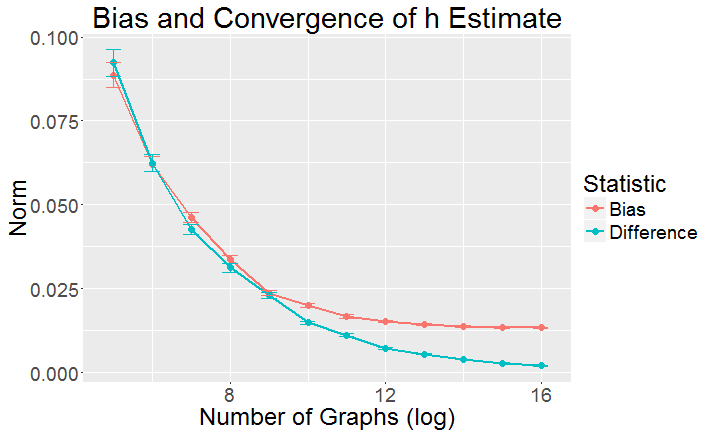
\includegraphics[scale=0.6,width=3.0in]{biasandconv.png}
	\caption{Bias and Convergence of Joint Embedding}
	%\label{fig:awesome_image}
\end{figure}

\noindent From the plot, we can see that the norm difference converges to $0$ as $m$ increases. It suggests the convergence of $\hat{h}_1^m$. Secondly, we should notice that the bias $\|\hat{h}^m_1-h_1\|$ does not converge to $0$; instead, it stops to decrease at around $0.03$. This suggests that $\hat{h}_1$ is an asymptotically biased estimator for $h_1$. The $\hat{h}_1^m$ with $m=2^{16}$ is $[0.083,0.186, 0.296, 0.406, 0.503]^T/0.74$. Compared to $h_1$, there are negative biases for small entries of $h_1$, and positive biases for large entries of $h_1$. Actually, there are some theoretical evidences for this phenomenon as well. In fact, when there are infinitely many nuisance parameters present, Neyman and Scott gives an example that maximum likelihood estimator can be inconsistent as well \cite{neyman1948consistent}. In our case, there are infinitely many $\lambda_i$s; therefore, we do not expect joint embedding to be an consistent estimator. \\

\noindent In applications like clustering or classifying multiple graphs, we may be not interested in $\hat{h}_1$. We are more interested in $\hat{\lambda}_i$ which provides information specifically about graph $G_i$. Here we consider two approaches to estimate $\lambda_i$. The first approach is estimating $\lambda_i$ through joint embedding,
\[ \hat{\lambda}_i = \langle A_i,  \hat{h}^m_1 \hat{h}^{m T}_1 \rangle \]
The second approach estimates $\lambda_i$ by forcing $\hat{h}_1$ equal to $h_1$, that is 
\[ \hat{\lambda}_i = \langle A_i,  h_1 h_1^T \rangle \]
$\hat{\lambda}_i$ calculated this way can be thought of as 'oracle' estimates, since it assumes $h_1$ is known. For each value of m, we provide a boxplot shows the differences in estimates provided by two approaches. Not surprisingly, the differences are small due to the fact that $\hat{h}_1^m$ and $h_1$ are close.
\begin{figure}[!htbp]
	\centering
	\includegraphics[scale=0.6,width=3.0in]{lambda_differ.png}
	\caption{Boxplot for Lambda Estimates}
	%\label{fig:awesome_image}
\end{figure}

\subsection{Simulation Experiment 2: Joint Embedding to Classify Graphs}
In this experiment, we consider the inference task of classifying graphs.  The set up is $m$ pairs $\{(A_i,Y_i)\}_{i=1}^{m}$ are observed. Each pair consists of an adjacency matrix $A_i \in \{0,1\}^{n \times n}$ and a label $Y_i \in [K]$. Furthermore, all pairs are assumed to be independent and identically distributed according to an unknown distribution $\mathbb{F}_{A,Y}$, that is
\[(A_1,Y_1),(A_2,Y_2),...,(A_m,Y_m) \overset{i.i.d.}{\sim} \mathbb{F}_{A,Y} \] 
The goal is to find a classifier $g$ which is a function $g:\{0,1\}^{n \times n} \rightarrow [K]$ which has small classification error $L_g=P(g(A)\neq Y)$. \\ 

\noindent We consider a binary classification problem where $Y$ can only take value $0$ or $1$. We independently generate $200$ graphs with 100 vertices from two MREG models each. Let $h_1$ and $h_2$ be two vectors in $\mathbb{R}^{100}$, and \[h_1=[0.1,...,0.1]^T \text{ , and } h_2=[-0.1,...,-0.1,0.1,...,0.1]^T \] 
Here, $h_2$ has $-0.1$ as its first 50 entries and $0.1$ as its last 50 entries. Conditioned on the value of $Y$, we generate graphs according to two MREG models, that is 
\[A_i|Y_i=0 \sim MREG(F_0,h_1,h_2) \text{ , with } F_0= \mathbbm{1}_{[25,5]} \]
\[A_i|Y_i=1 \sim MREG(F_1,h_1,h_2) \text{ , with } F_1= \mathbbm{1}_{[22.5,2.5]} \]
In terms of SBM, this graph generation scheme is also equivalent to,
\[ A_i|Y_i=0 \sim  SBM((1,...,1,2,...,2),\begin{bmatrix} 0.3 & 0.2 \\ 0.2 & 0.3 \\ \end{bmatrix})  \]
\[ A_i|Y_i=1 \sim  SBM((1,...,1,2,...,2),\begin{bmatrix} 0.25 & 0.2 \\ 0.2 & 0.25 \\ \end{bmatrix})\]

\noindent To classify graphs, we first jointly embed $200$ graphs. The embeddings are shown in the figure below. We can see two classes are clearly separated after being jointly embedded.
\begin{figure}[!htbp]
	\centering
	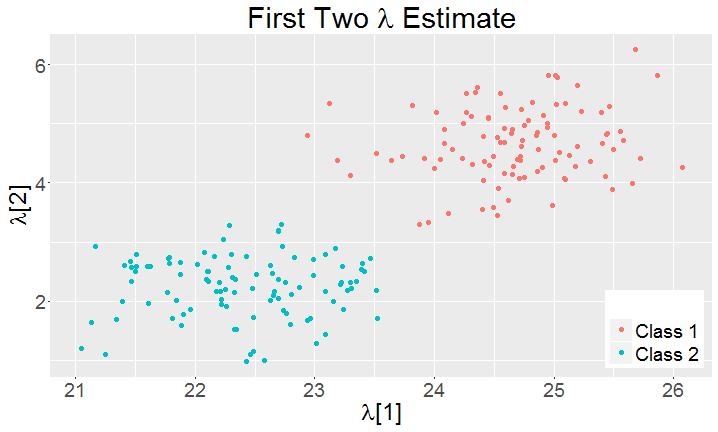
\includegraphics[scale=0.6,width=3.0in]{JE_200.png}
	\caption{$\Lambda_i$ of jointly embedded graphs}
	%\label{fig:awesome_image}
\end{figure}
Then, an 1-nearest neighbor classifier is constructed based on loadings $\{\hat{\lambda}_i\}_{i=1}^m$. The 1-NN classification error with $200$ graphs is $0$. \\
\\
\noindent We compare classification performance using joint embedding and laplacian eigenmap \cite{belkin2003laplacian}. For laplacian eigenmap, we first embed each normalized laplacian matrix and then compute Frobenious norm between embeddings. We also apply a 1-NN rule to classify graphs. We let the number of graphs $m$ to increase from $4$ to $200$. For each value of $m$, we repeat the simulation $100$ times. The result is shown in the next figure. We see joint embedding takes advantage of increasing sample size and dominates ASE at all values of $m$. 
\begin{figure}[!htbp]
	\centering
	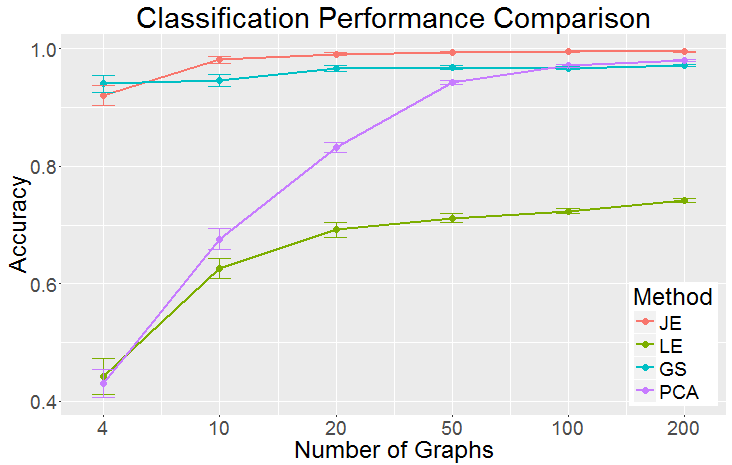
\includegraphics[scale=0.6,width=3.0in]{leig_je_acc.png}
	\caption{Classification Performance of Joint Embedding and ASE}
	%\label{fig:awesome_image}
\end{figure} 




\subsection{Real Data Experiment: CCI}
In this experiment, we consider predicting individual composite creativity index (CCI) through functional (structural???) magnetic resonance imaging. Neuroimaging and creativity have been jointly investigated previously \cite{arden2010neuroimaging}. Most of studies utilize a statistical testing method and find CCI significant related or inversely related to the activity of some regions of brain. We embrace a different approach by finding a regression model for CCI. We first jointly embed brain images and then regress CCI loadings estimated.

\noindent 113 healthy, young adult subjects were scanned on using (???) scanner with functional magnetic resonance imaging. The image is then registered by Desikan atlas(???) \cite{desikan2006automated} and a graph of 70 vertices is constructed through computing pairwise correlations across regions. DT measures were scored by (???) independent judges using the Consensual Assessment Technique \cite{amabile1983social}, from which a CCI was derived. To predict CCI, we jointly embed 113 graphs with $d=10$. Then, we construct a linear regression model by treating CCI as the response variable and $\hat{\lambda}_i$ as predictors, that is
\[CCI_i \sim \beta_0+\lambda_i^T\beta + \epsilon_i \]
If only $\hat{\lambda}_i[1]$ is used as predictor, the figure \ref{fig:cci} shows the result. We can see a linear relationship between CCI and first dimension loadings. If fit CCI to all the loadings, a summary of the linear model is provided in appendix. The R-square is $0.2325$ and the model is statistically significant better compared to the null model with a p-value $0.0018$. 
\begin{figure}[!htbp]
	\centering
	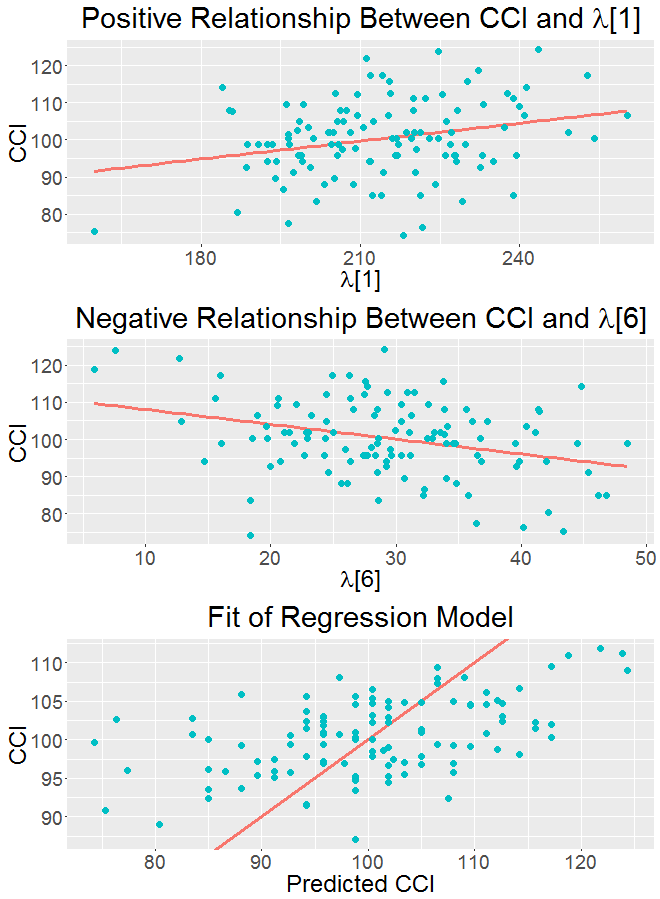
\includegraphics[scale=0.6,width=3.0in]{cci.png}
	\caption{Predicting Creativity Index with Joint Embeddings}
	\label{fig:cci}
\end{figure}



\section{conclusion}
In summary, we develop a joint embedding method which can simultaneously embed multiple graphs into low dimensional space. Joint embedding can
be used to estimate simple and intuitive statistics for inference problems on multiple vertex matched graphs. Learning on multiple graphs has significant applications in diverse fields and our results have both theoretical and practical implications for the problem. As the real data experiment illustrate, joint embedding is a practically viable inference procedure. \\

\noindent We also propose a Multiple Random Eigen Graphs model. It can be seen as a generalization of random dot product graph model or stochastic block model for multiple random graphs. We analyze the performance of joint embedding on this model under simple settings. It can be shown our method provides estimates with bounded error. \\

\noindent Our approach is intimately related other matrix factorization approaches like singular value decomposition and tensor factorization. Indeed, they all try to estimate a low dimensional representation of high dimensional objects. We are currently investigate joint embedding with more or less regularizations on parameters under difference real set ups.  

\appendix
\begin{proof} [Proof of Theorem 4.1]
First,  we are going to show that $|D_n(h,h_1)-D(h,h_1)|$ converges uniformly to $0$.
We notice three facts,
\begin{itemize}
	\item[(1)] The set $\{h: \|h\|=1\}$ is a compact set.
	\item[(2)] The function $\rho(A_i,h)$ is continuous for all $h$.
	\item[(3)] For all $h$, $\rho(A_i,h)$ is bounded by $n^2$.
\end{itemize}
Therefore, by the uniform law of large numbers \cite{jennrich1969asymptotic}, we have
\[\underset{h}{\sup}|D_m(h,h_1)-D(h,h_1)|\overset{a.s.}{\rightarrow} 0\]
To prove the claim of theorem, we use a similar technique employed by Bickel and Doksum \cite{bickel2015mathematical}. By definition, we have $D_m(\hat{h}_1^m,h)  \leq D_m(h',h)$ and $D(h',h) \leq D(\hat{h}_1^m,h)$. Using these two inequalities we have
\begin{align*}
D_m(h',h)-D(h',h) &\geq D_m(\hat{h}_1^m,h)-D(h',h) \\
&\geq D_m(\hat{h}_1^m,h)-D(\hat{h}_1^m,h) 
\end{align*}
Therefore, 
\begin{align*}
|D_m(\hat{h}_1^m,h)-D(h',h)|  \leq  \max(&|D_m(h',h)-D(h',h)|,\\
& |D_m(\hat{h}_1^m,h)-D(\hat{h}_1^m,h)|)
\end{align*}
This implies 
\[ |D_m(\hat{h}_1^m,h)-D(h',h)| \leq \underset{h}{\sup}|D_m(h,h_1)-D(h,h_1)| \]
Hence, $|D_m(\hat{h}_1^m,h)-D(h',h)|$ must converge almost surely to $0$ ,that is
\[|D_m(\hat{h}_1^m,h)-D(h',h)|\overset{a.s.}{\rightarrow} 0 \]
 If $\hat{h}_1^m$ does not converge almost surely $h'$, $\|\hat{h}_1^m-h'\|\geq \epsilon$ for some $\epsilon$ and infinitely many values of $m$. Since $h'$ is the unique global minimum, $|D(\hat{h}_1^m,h)-D(h',h)| > \epsilon' $ for infinitely many values of $m$. This contradicts with the previous equation. Therefore, $\hat{h}_1^m$ must converges almost surely $h'$.
	
\end{proof}


\begin{proof} [Proof of Theorem 4.2]
The first part of proof is showing that $h'$ is the eigenvector corresponds to the largest eigenvalue of $E(\langle A_{i},h' h'^T \rangle A_{i})$. Then, we show $E(\langle A_{i},h' h'^T \rangle A_{i})$ is close to a properly scaled $E(P_i)$. To conclude, we apply Davis-Kahan theorem to the top eigenvector of both matrices and get the desired result. First, we notice that
	\begin{align*}
	\underset{\|h\| =1}{\operatorname{min}}D(h,h_1) &=\underset{\|h\| =1}{\operatorname{min}}E(\|A_i- \langle A_i,h h^T \rangle h h^T\|^2) \\
	&=\underset{\|h\| =1}{\operatorname{min}}E(\langle A_i,A_i \rangle- \langle A_i,h h^T \rangle ^2) \\
	&=E(\langle A_i,A_i \rangle)-\underset{\|h\| =1}{\operatorname{max}}E( \langle A_i,h h^T \rangle ^2)
	\end{align*}
	Therefore, 
	\begin{equation} \label{eq:5}
	h'= \underset{\|h\| =1}{\operatorname{argmin}} \text{ }D(h,h_1)=\underset{\|h\| =1}{\operatorname{argmax}} \text{ } E(\langle A_i,h h^T \rangle ^2) 
	\end{equation}
	Taking the derivative of $E( \langle A_i,h h^T \rangle ^2)+ c(h^Th-1)$ with respect to $h$, we have 
	\begin{align*}
	\frac{\partial E( \langle A_i,h h^T \rangle ^2)+ c(h^Th-1) }{\partial h} & =  E(\frac{\partial  \langle A_i,h h^T \rangle ^2}{\partial h}) +2ch \\
	&=4 E( \langle A_i,h h^T \rangle A_i)h +2ch 
	\end{align*}
	Set it to $0$,
	\begin{align*} 
	E( \langle A_i,h' h'^T \rangle A_i)h' & = -\frac{1}{2}ch' 
	\end{align*}
	Using the fact that, $\|h'\|=1$, we can solve $c$
	\[ h'^T E( \langle A_i,h' h'^T \rangle A_i)h' = E( \langle A_i,h' h'^T \rangle^2)= -\frac{1}{2}c \]
	Then, substitute $c$
	\begin{equation}
	E( \langle A_i,h' h'^T \rangle A_i)h'=E( \langle A_i,h' h'^T \rangle^2)h'
	\end{equation}
	Therefore, we see $h'$ is an eigenvector of $E(\langle A_{i},h' h'^T \rangle A_{i})$ and the corresponding eigenvalue is $E(\langle A_{i},h' h'^T \rangle ^2)$. Furthermore, $E(\langle A_{i},h' h'^T \rangle ^2)$ must be the eigenvalue with the largest magnitude. Assume not, then there exists a $h''$ with norm 1 such that
	\begin{align*}  | h''^T E(\langle A_{i},h' h'^T \rangle A_{i}) h''| &= |E(\langle A_{i},h' h'^T \rangle \langle A_{i},h'' h''^T \rangle)| \\
	&> E(\langle A_{i},h' h'^T \rangle ^2)  、
	\end{align*}
	However, by Cauchy-Schwarz inequality we must have
	\begin{align*} E(\langle A_{i},h'' h''^T \rangle^2)  E(\langle A_{i},h' h'^T \rangle^2) &> \\
	&|E(\langle A_{i},h' h'^T \rangle \langle A_{i},h'' h''^T \rangle)|^2 
	\end{align*}
	This implies $E(\langle A_{i},h'' h''^T \rangle^2) > E(\langle A_{i},h' h'^T \rangle^2)$ which contradicts equation \eqref{eq:5}. This concludes that $h'$ is the eigenvector corresponds to the largest eigenvalue of $E(\langle A_{i},h' h'^T \rangle A_{i})$. \\
	
	\noindent Next, we compute $E(\langle A_{i},h' h'^T \rangle A_{i})$.
	\begin{align*}
	&E(\langle A_{i},h' h'^T \rangle A_{i}|P_i)    \\
	&=E( \langle A_{i}-P_i,h' h'^T \rangle (A_{i}-P_i)|P_i)\\
	&\qquad {}+E(\langle A_{i}-P_i,h' h'^T \rangle P_i)|P_i) \\
	&\qquad {} +E(\langle P_i,h' h'^T \rangle (A_{i}-P_i)|P_i)+E(\langle P_i,h' h'^T \rangle P_i|P_i) \\
	&= E(\langle A_{i}-P_i,h' h'^T \rangle (A_{i}-P_i)|P_i) + \lambda_i (h_1^Th')^2 P_i \\
	&=  2h' h'^T *P_i*(J-P_i) - DIAG(h_1 h_1^T *P_i*(J-P_i)) 	\\
	&\qquad {}+\lambda_i (h_1^Th')^2 P_i 
	\end{align*}
	Here, DIAG() means only keep the diagonal of matrix; $*$ means the Hadamard product, and $J$ is a matrix of all ones. Using the fact that $P_i=\lambda_i h_1 h_1 ^T$, we have 
	\begin{align*}
	&E(\langle A_{i},h' h'^T \rangle A_{i}) - E(\lambda_i^2) (h_1^Th')^2 h_1 h_1^T \\
	&=E(E(\langle A_{i},h' h'^T \rangle A_{i}|P_i)-\lambda_i (h_1^Th')^2 P_i) 
	 \\
	&= E(2 h' h'^T *P_i*(J-P_i) - DIAG(h' h'^T*P_i*(J-P_i)))
	\end{align*}
	If we consider the norm difference between $E( \langle A_{i},h' h'^T \rangle A_{i})$ and $ E(\lambda_i^2) (h_1^Th')^2 h_1 h_1^T$, we have
	\begin{align*}
	&\|E(\langle A_{i},h' h'^T \rangle A_{i} ) - E(\lambda_i^2) (h_1^Th')^2 h_1 h_1^T\| \\
	&= \|E(2 h' h'^T *P_i*(J-P_i) - DIAG(h' h'^T*P_i*(J-P_i)))\| \\
	&\leq  E(\|2 h' h'^T *P_i*(J-P_i) - DIAG(h' h'^T*P_i*(J-P_i))\|) \\
	&\leq  E(\|2 h' h'^T *P_i*(J-P_i)\|) \\
	&\leq  E(\|2 h' h'^T * P_i\|) \\
	&\leq  2 E(\lambda_i)\| h' h'^T * h_1 h_1^T\| \\
	&=  2 E(\lambda_i) 
	\end{align*}
	Notice that the only non-zero eigenvector of $E(\lambda_i^2) (h_1^Th')^2 h_1 h_1^T$ is $h_1$ and the corresponding eigenvalue is $E(\lambda_i^2) (h_1^Th')^2$. We apply Davis-Kahan theorem \cite{davis1970rotation} to the eigenvector corresponding to the largest eigenvalue of matrices $E(\langle A_{i},h' h'^T \rangle A_{i} )$ and $E(\lambda_i^2) (h_1^Th')^2 h_1 h_1^T$,
	\[\|h'-h_1\| \leq \frac{2 E(\lambda_i)}{E(\lambda_i^2)(h_1^T h')^2} \]
\end{proof}

\noindent{\bf CCI Linear Model Summary}
\begin{lstlisting}
> model<-lm(cci~Lambda+1)
> summary(model)

Call:
lm(formula = cci ~ Lambda + 1)

Residuals:
Min       1Q   Median     3Q    Max 
-26.3432 -6.144 -0.7578 7.1032  16.9004 

Coefficients: Estimate  Pr(>|t|)    
(Intercept)  1.275e+02   0.000275 ***
Lambda1      2.421e-04   0.997981    
Lambda2     -2.326e-01   0.070110 .  
Lambda3     -3.716e-02   0.822592    
Lambda4      8.049e-02   0.687628    
Lambda5     -2.925e-01   0.421858    
Lambda6     -4.285e-01   0.009088 ** 
Lambda7     -1.745e-01   0.590533    
Lambda8     -3.465e-01   0.240093    
Lambda9     -8.970e-01   0.007999 ** 
Lambda10    -8.955e-01   0.052839 .  
---
Signif. codes:  0 ‘***’ 0.001 ‘**’ 
0.01 ‘*’ 0.05 ‘.’ 0.1 ‘ ’ 1

Residual standard error: 9.437 
on 102 degrees of freedom,
Multiple R-squared:  0.2325,
Adjusted R-squared:  0.1572 
F-statistic:  3.09 on 10 and 102 DF,  
p-value: 0.001795
\end{lstlisting}

% references section

% can use a bibliography generated by BibTeX as a .bbl file
% BibTeX documentation can be easily obtained at:
% http://mirror.ctan.org/biblio/bibtex/contrib/doc/
% The IEEEtran BibTeX style support page is at:
% http://www.michaelshell.org/tex/ieeetran/bibtex/
%\bibliographystyle{IEEEtran}
% argument is your BibTeX string definitions and bibliography database(s)
%\bibliography{IEEEabrv,../bib/paper}
%
% <OR> manually copy in the resultant .bbl file
% set second argument of \begin to the number of references
% (used to reserve space for the reference number labels box)
\bibliographystyle{IEEEtran}
\bibliography{citations}



% biography section
% 
% If you have an EPS/PDF photo (graphicx package needed) extra braces are
% needed around the contents of the optional argument to biography to prevent
% the LaTeX parser from getting confused when it sees the complicated
% \includegraphics command within an optional argument. (You could create
% your own custom macro containing the \includegraphics command to make things
% simpler here.)
%\begin{IEEEbiography}[{\includegraphics[width=1in,height=1.25in,clip,keepaspectratio]{mshell}}]{Michael Shell}
% or if you just want to reserve a space for a photo:

%\begin{IEEEbiography}{Shangsi Wang}
%Biography text here.
%\end{IEEEbiography}

% if you will not have a photo at all:
%\begin{IEEEbiographynophoto}{Carey Priebe}
%Biography text here.
%\end{IEEEbiographynophoto}

% insert where needed to balance the two columns on the last page with
% biographies
%\newpage




\end{document}



